\documentclass[12pt,a4paper]{report}

%--------------------------------------
\usepackage[T1]{fontenc} %Not needed by LuaLaTeX or XeLaTeX
%--------------------------------------

%Portuguese-specific commands
%--------------------------------------
%\usepackage[portuguese]{babel}
%--------------------------------------

%Hyphenation rules
%--------------------------------------
\usepackage{hyphenat}
\hyphenation{mate-mática recu-perar}
%--------------------------------------

%Espaçamento e outras cenas
%--------------------------------------
\usepackage{setspace}
\usepackage{anyfontsize}
\usepackage{indentfirst}
\usepackage{parskip}
\usepackage{titlesec} % Chapter
\usepackage{geometry} % Margens
\usepackage{amsmath} % Matemática
\usepackage{graphicx}
\usepackage{wrapfig}
\usepackage{subcaption}
\usepackage{caption}
\usepackage[hidelinks]{hyperref}
\usepackage{xpatch}
\usepackage{etoolbox}
\usepackage{titletoc}
\usepackage{times}
\usepackage{fancyhdr}
\usepackage{lastpage}
\usepackage{xcolor}
\usepackage{listings}
%------------------------------

%Margens
\geometry{
    a4paper,
    right = 3cm,
    left = 2.5cm,
    top = 2.5cm,
    bottom = 2.5cm,
}

\renewcommand{\contentsname}{Índice}
\newcommand{\code}{\texttt\textbf}

\setcounter{secnumdepth}{0} % Não enumerar secções

\setstretch{1.5} % espaçamento

\titleformat{\chapter}{\fontfamily{ptm}\selectfont\centering\huge\titlerule[1.5pt]\vspace{-9pt}}{}{0pt}{\Huge}[{\titlerule[1.5pt]}]

\titleformat{\section}{\bfseries\fontfamily{ptm}\selectfont}{}{0pt}{\large}[{\titlerule[1pt]}]

\titlespacing{\chapter}{0pt}{-30pt}{30pt}


\titlecontents{section}[40pt]{\vskip3pt\bfseries}{\thecontentslabel\quad}{}{~~\normalfont\dotfill\bfseries\contentspage}[]


\begin{document}


\chapter{Introdução}

Quando estamos perante uma situação na qual temos de lidar com a manipulação de grandes quantidades de dados existem sempre algumas opções que devemos preferir adotar e outras que pelo contrário devemos evitar a todo o custo, portanto ao longo deste relatório iremos explicar as estratégias que utilizámos para abordar este problema e porque razão optámos por uma estratégia em específico e não outra qualquer.

Posto isto, importa também realçar que nas estruturas que iremos exemplificar mais à frente tivemos em conta a natureza dos dados com os quais estávamos a lidar e as questões que tinham de ser resolvidas em tempo útil, assim sendo, caso levássemos em conta outros quaisquer fatores certamente a abordagem adotada teria sido outra.

\chapter{Catálogos}

Antes de mais, a primeira etapa do projeto diz respeito ao armazenamento dos dados, ou seja, tínhamos de guardar toda a informação útil numa determinada estrutura de dados, portanto como reparámos que existem três entidades fundamentais \textit{(users, drivers, rides)}, decidimos criar uma estrutura de dados para cada uma destas entidades e mais uma para as cidades, visto que em várias \textit{queries} as cidades são um dos parâmetros visados.

\section{Utilizadores}

\begin{figure}[h]
    \centering
    \begin{subfigure}{\textwidth}
        \centering
        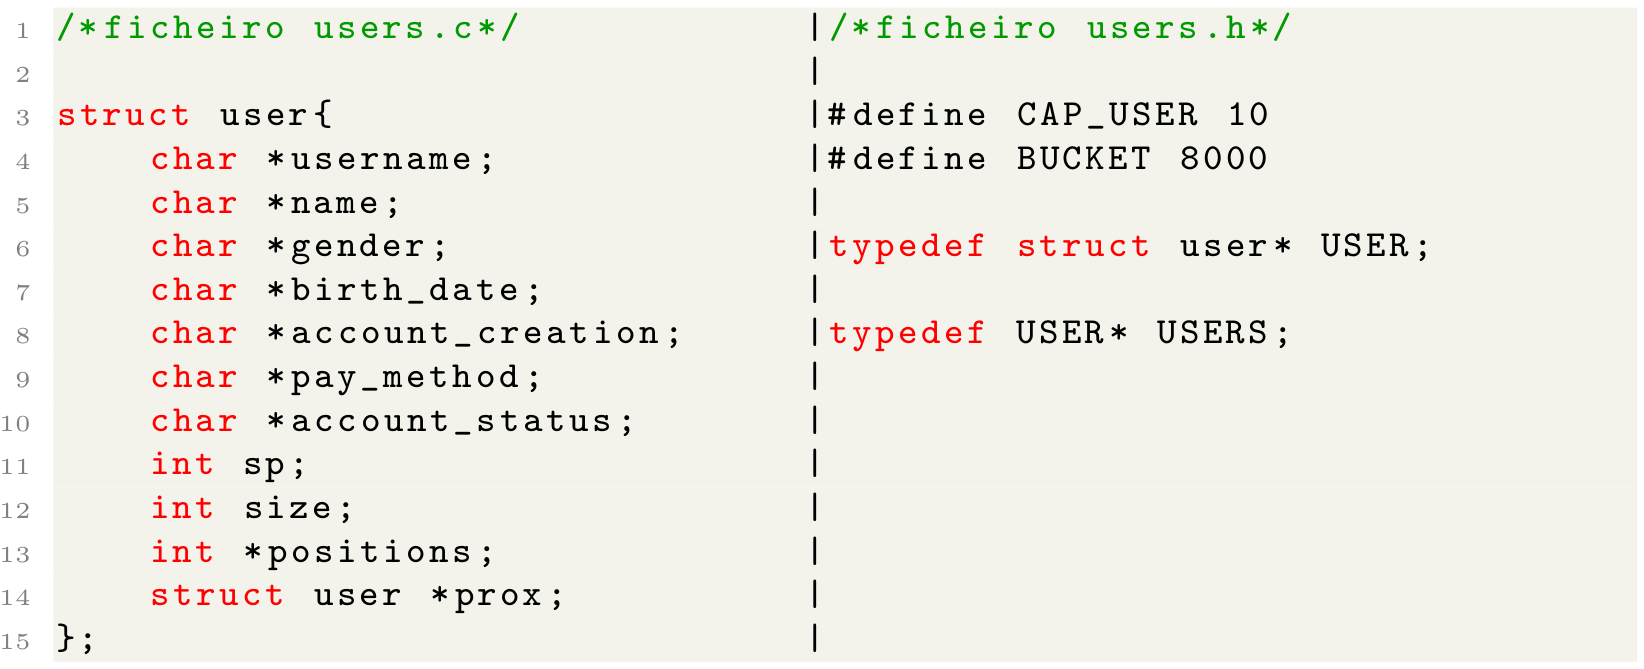
\includegraphics[width=1\linewidth]{images/users.png}
        \caption*{Estrutura de dados dos utilizadores}
        \label{fig:users}
    \end{subfigure}
\end{figure}

Tal como é possível observar pela estrutura presente no ficheiro \textit{users.c}, é possível depreender que um utilizador é um elemento de uma lista ligada, visto que um dos campos corresponde a um apontador para outro \texttt{\small\textbf{struct user}}, além disso, existe mais um campo em particular para além daqueles que como estão presentes no ficheiro \textit{csv} também teria de estar contidos aqui, falamos nem mais nem menos do campo \texttt{\small\textbf{positions}}, este parâmetro representa um \textit{array} dinâmico que começa com tamanho que é definido por \textbf{\small\texttt{CAP\_USER}}, e que depois vai multiplicado por dois à medida que o valor de \texttt{\small\textbf{sp}} iguala o valor do \small\texttt{\textbf{size}}, sendo que \texttt{\small\textbf{sp}} representa o número de elementos que o \textit{array} dinâmico \texttt{\small\textbf{positions}} possui, por fim o \textit{array} \texttt{\small\textbf{positions}} possui todas as posições em que um determinado utilizador aparece no \textit{array} das viagens.

Passando para o ficheiro \textit{users.h} percebe-se de que forma os utilizadores estão organizados, neste caso os utilizadores são guardados numa tabela de \textit{hash}, em que cada utilizador é mapeado para uma determinada posição conforme o seu \texttt{\small\textbf{username}} e é acrescentado no início da lista ligada para poupar o máximo de tempo possível, assim a estrutura \texttt{\small\textbf{USERS}} representa uma tabela de \textit{hash} com 8000 \textit{buckets}, onde cada utilizador pode ser acedido em tempo praticamente constante (não sendo constante pois é necessário percorrer a lista ligada de um determinado \textit{bucket} até encontrar o \texttt{\small\textbf{username}} que pretendemos).



\normalsize\textbf{Vantagens}
    \begin{enumerate}
        \item Ao utilizar uma tabela de \textit{hash} podemos encontrar um utilizador mais facilmente uma vez que a função de \textit{hash} mapeia apenas para um determinado índice.

        \item Ao utilizar uma lista ligada em cada um dos \textit{buckets} é possível inserir um utilizador no início da lista de forma constante, algo que não seria possível num \textit{array}.
        
        \item Ao usufruir de uma lista ligada apenas vamos alocar a quantidade exata de memória que necessitamos para representar os nossos dados. 
    \end{enumerate}

\normalsize\textbf{Desvantagens}
    \begin{enumerate}
        \item A utilização de listas ligadas não tira partido na memória espacial, uma vez que o apontadores para os próximos elementos da lista estarão dispersos na memória, como tal, a \textit{miss rate} aumenta o portanto demora mais tempo a aceder ao elemento seguinte da lista ligada.
        
        \item Ao utilizar uma tabela de \textit{hash} vai ser desperdiçado bastante tempo para libertar a memória que foi necessária alocar anteriormente, visto que teremos que percorrer cada uma das listas ligadas presentes na tabela de \textit{hash}.
    \end{enumerate}

\pagebreak
\section{Condutores}

\begin{figure}[hbt!]
    \centering
    \begin{subfigure}{\textwidth}
        \centering
        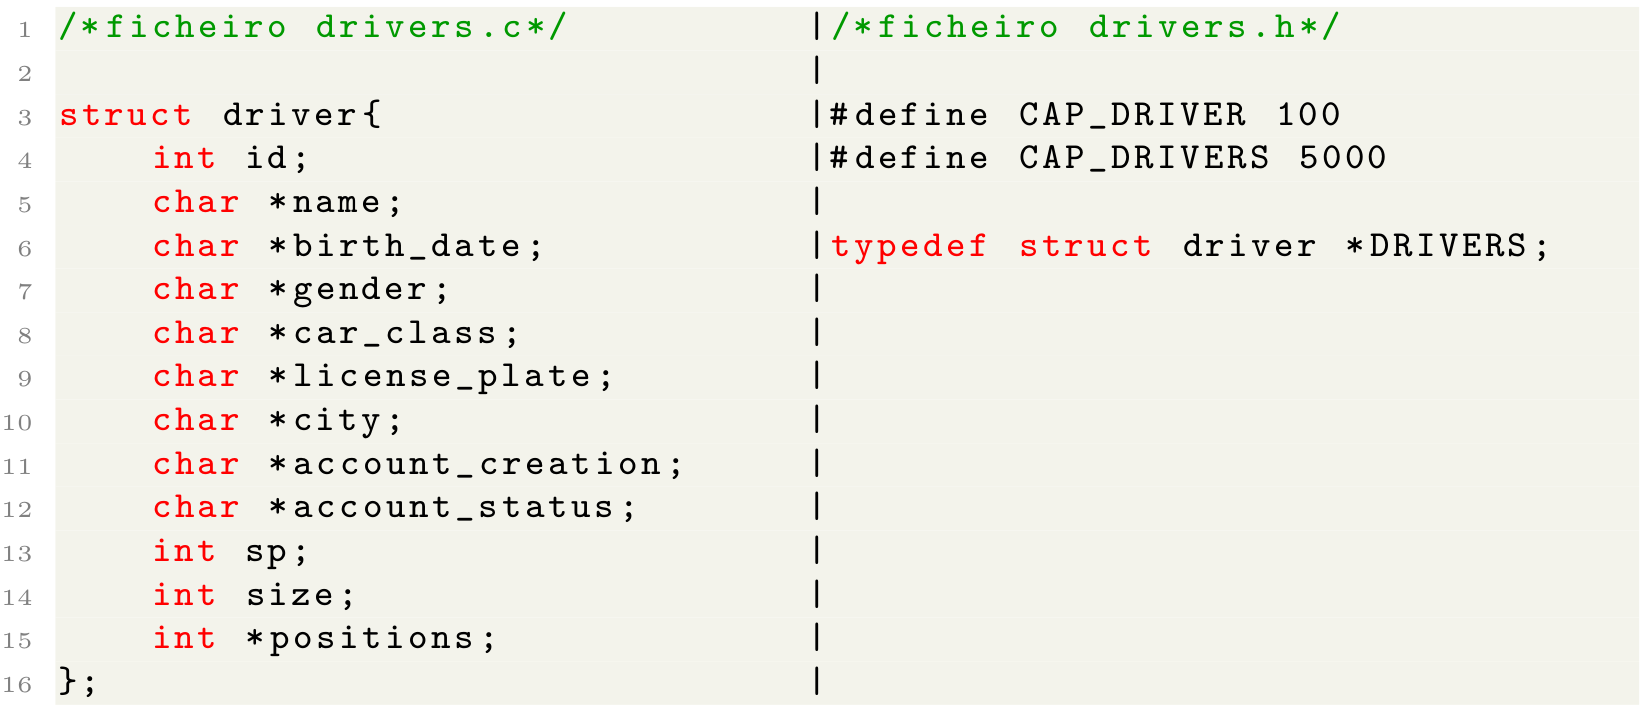
\includegraphics[width=1\linewidth]{images/drivers.png}
        \caption*{Estrutura de dados dos condutores}
        \label{fig:drivers}
    \end{subfigure}
\end{figure}

Agora na estrutura dos condutores, a estratégia adotada foi muito parecida à dos utilizadores, mais uma vez, todos os campos que estão presentes nos ficheiro \textit{drivers.csv} também estão aqui presentes, e além disso também existe outro \textit{array} dinâmico \textbf{\small\texttt{positions}} que a exemplo do anterior possui um tamanho inicial definido por \textbf{\small\texttt{CAP\_DRIVER}}, e tem como elementos todas as posições que um determinado condutor aparece no \textit{array} das viagens.

De seguida, ao analisar o ficheiro \textit{drivers.h}, vemos que a estrutura \textbf{\small\texttt{DRIVERS}} é um \textit{array} dinâmico de tamanho inicial definido por \textbf{\small\texttt{CAP\_DRIVERS}}, onde cada elemento é um condutor. Neste caso a forma de mapeamento utilizada para colocar um determinado condutor numa posição do \textit{array} foi o \textbf{\small\texttt{id}} do condutor, ou seja, um condutor com um \textbf{\small\texttt{id}} correspondente a \textbf{\small\texttt{000000000162}} será mapeado na posição de índice \textbf{\small\texttt{162}} do \textit{array} \textbf{\small\texttt{DRIVERS}}.


\normalsize\textbf{Vantagens}
    \begin{enumerate}
        \item A utilização de um \textit{array} tira partido da localidade espacial, o que aumenta o \textit{hit rate}, e consequentemente leva a um ganho de tempo caso pretendamos percorrer o \textit{array} de início a fim.
        
        \item Ao utilizar um \textit{array} dinâmico, nunca corremos o risco de alocar demasiada memória do que aquela de é extremamente necessária, no pior dos casos alocamos o dobro daquela que seria pretendida.
        
        \pagebreak
        \item Quando pretendemos libertar a memória do \textit{array} \textbf{\small\texttt{DRIVERS}} não vai ser necessário percorrer o \textit{array}, ao contrário da tabela de \textit{hash}, neste caso a operação de libertar memória será feita em tempo constante.
        
        \item Se pretende aceder a um determinado utilizador, é possível fazer essa operação em tempo constante desde que saiba qual o \textbf{\small\texttt{id}} do condutor em questão.
    \end{enumerate}

\normalsize\textbf{Desvantagens}
    \begin{enumerate}
        \item A menos que saibamos qual o índice de um determinado condutor no \textit{array} \textbf{\small\texttt{DRIVERS}}, teremos de percorrer o \textit{array} até encontrar o condutor que pretendemos.

        \item Ao utilizar esta forma de mapear um condutor no \textit{array} \textbf{\small\texttt{DRIVERS}} a posição de índice zero está sempre vazia uma vez que nenhum condutor tem um \textbf{\small\texttt{id}} igual a zero.
    \end{enumerate}


\end{document}